% !WASMTEX tikz-externalization = auto
% Phase 6.1 fixture for docs/plans/2026-11-12-latex-compile-cost.md: twelve
% TikZ pictures between paragraphs, so a text edit can be measured with and
% without TikZ externalization. No \tikzexternalize: the 'auto' mode is what
% activates it.
\documentclass[11pt]{article}
\usepackage{fontspec}
\setmainfont{Latin Modern Roman}
\usepackage{tikz}
\usepackage[margin=2.5cm]{geometry}

\begin{document}
\section{Introduction}
Performance probe paragraph T1. This document measures how a text edit
behaves when the document is full of TikZ pictures.

\section{Figure 1}
Paragraph before figure 1. The picture below is drawn with TikZ: a regular
polygon with 5 sides, a grid, a labelled node and an arrow.

\begin{figure}[h]
  \centering
  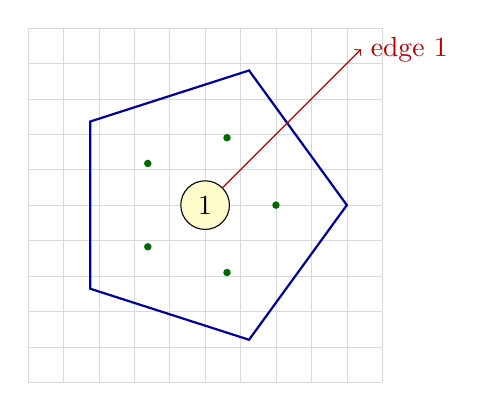
\begin{tikzpicture}[scale=0.9]
    \draw[step=0.5, gray!30, very thin] (-2.5,-2.5) grid (2.5,2.5);
    \draw[thick, blue!60!black] (2.00,0.00) -- (0.62,1.90) -- (-1.62,1.18) -- (-1.62,-1.18) -- (0.62,-1.90) -- cycle;
    \node[draw, circle, fill=yellow!20] (c1) at (0,0) {1};
    \draw[->, red!70!black] (c1) -- (2.2,2.2) node[right] {edge 1};
    \foreach \x in {1,...,5} { \fill[green!40!black] (\x*360/5:1) circle (1.5pt); }
  \end{tikzpicture}
  \caption{TikZ figure 1.}
  \label{fig:tikz:1}
\end{figure}

Paragraph after figure 1, referring to Figure~\ref{fig:tikz:1}.

\section{Figure 2}
Paragraph before figure 2. The picture below is drawn with TikZ: a regular
polygon with 6 sides, a grid, a labelled node and an arrow.

\begin{figure}[h]
  \centering
  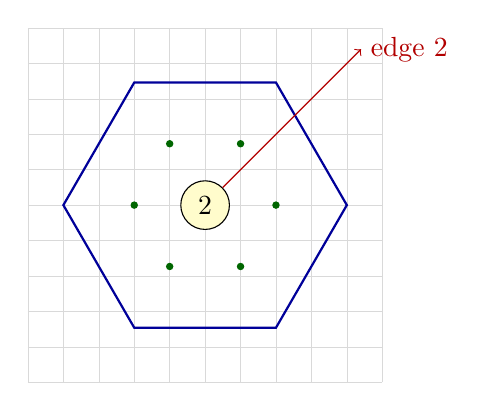
\begin{tikzpicture}[scale=0.9]
    \draw[step=0.5, gray!30, very thin] (-2.5,-2.5) grid (2.5,2.5);
    \draw[thick, blue!60!black] (2.00,0.00) -- (1.00,1.73) -- (-1.00,1.73) -- (-2.00,0.00) -- (-1.00,-1.73) -- (1.00,-1.73) -- cycle;
    \node[draw, circle, fill=yellow!20] (c2) at (0,0) {2};
    \draw[->, red!70!black] (c2) -- (2.2,2.2) node[right] {edge 2};
    \foreach \x in {1,...,6} { \fill[green!40!black] (\x*360/6:1) circle (1.5pt); }
  \end{tikzpicture}
  \caption{TikZ figure 2.}
  \label{fig:tikz:2}
\end{figure}

Paragraph after figure 2, referring to Figure~\ref{fig:tikz:2}.

\section{Figure 3}
Paragraph before figure 3. The picture below is drawn with TikZ: a regular
polygon with 7 sides, a grid, a labelled node and an arrow.

\begin{figure}[h]
  \centering
  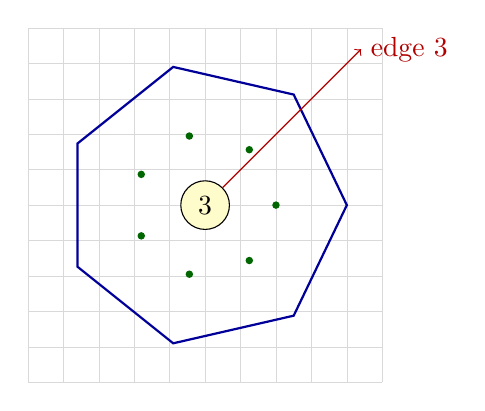
\begin{tikzpicture}[scale=0.9]
    \draw[step=0.5, gray!30, very thin] (-2.5,-2.5) grid (2.5,2.5);
    \draw[thick, blue!60!black] (2.00,0.00) -- (1.25,1.56) -- (-0.45,1.95) -- (-1.80,0.87) -- (-1.80,-0.87) -- (-0.45,-1.95) -- (1.25,-1.56) -- cycle;
    \node[draw, circle, fill=yellow!20] (c3) at (0,0) {3};
    \draw[->, red!70!black] (c3) -- (2.2,2.2) node[right] {edge 3};
    \foreach \x in {1,...,7} { \fill[green!40!black] (\x*360/7:1) circle (1.5pt); }
  \end{tikzpicture}
  \caption{TikZ figure 3.}
  \label{fig:tikz:3}
\end{figure}

Paragraph after figure 3, referring to Figure~\ref{fig:tikz:3}.

\section{Figure 4}
Paragraph before figure 4. The picture below is drawn with TikZ: a regular
polygon with 8 sides, a grid, a labelled node and an arrow.

\begin{figure}[h]
  \centering
  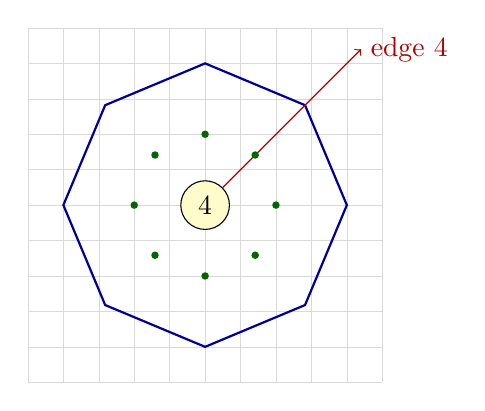
\begin{tikzpicture}[scale=0.9]
    \draw[step=0.5, gray!30, very thin] (-2.5,-2.5) grid (2.5,2.5);
    \draw[thick, blue!60!black] (2.00,0.00) -- (1.41,1.41) -- (0.00,2.00) -- (-1.41,1.41) -- (-2.00,0.00) -- (-1.41,-1.41) -- (-0.00,-2.00) -- (1.41,-1.41) -- cycle;
    \node[draw, circle, fill=yellow!20] (c4) at (0,0) {4};
    \draw[->, red!70!black] (c4) -- (2.2,2.2) node[right] {edge 4};
    \foreach \x in {1,...,8} { \fill[green!40!black] (\x*360/8:1) circle (1.5pt); }
  \end{tikzpicture}
  \caption{TikZ figure 4.}
  \label{fig:tikz:4}
\end{figure}

Paragraph after figure 4, referring to Figure~\ref{fig:tikz:4}.

\section{Figure 5}
Paragraph before figure 5. The picture below is drawn with TikZ: a regular
polygon with 4 sides, a grid, a labelled node and an arrow.

\begin{figure}[h]
  \centering
  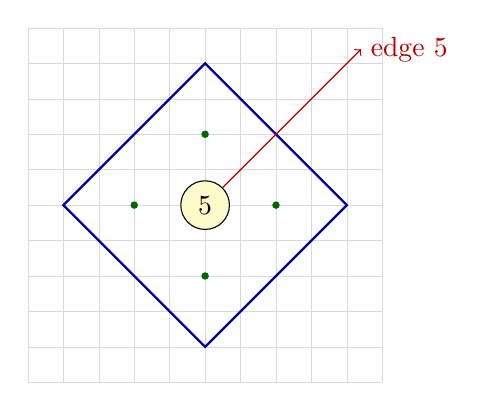
\begin{tikzpicture}[scale=0.9]
    \draw[step=0.5, gray!30, very thin] (-2.5,-2.5) grid (2.5,2.5);
    \draw[thick, blue!60!black] (2.00,0.00) -- (0.00,2.00) -- (-2.00,0.00) -- (-0.00,-2.00) -- cycle;
    \node[draw, circle, fill=yellow!20] (c5) at (0,0) {5};
    \draw[->, red!70!black] (c5) -- (2.2,2.2) node[right] {edge 5};
    \foreach \x in {1,...,4} { \fill[green!40!black] (\x*360/4:1) circle (1.5pt); }
  \end{tikzpicture}
  \caption{TikZ figure 5.}
  \label{fig:tikz:5}
\end{figure}

Paragraph after figure 5, referring to Figure~\ref{fig:tikz:5}.

\section{Figure 6}
Paragraph before figure 6. The picture below is drawn with TikZ: a regular
polygon with 5 sides, a grid, a labelled node and an arrow.

\begin{figure}[h]
  \centering
  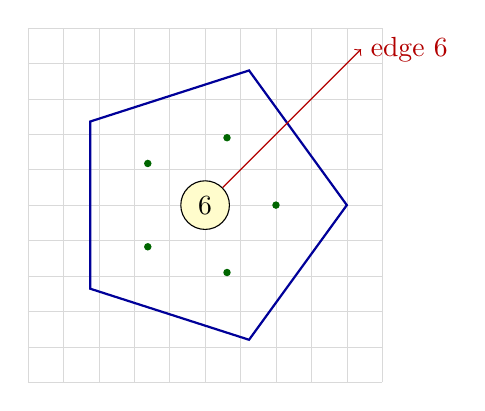
\begin{tikzpicture}[scale=0.9]
    \draw[step=0.5, gray!30, very thin] (-2.5,-2.5) grid (2.5,2.5);
    \draw[thick, blue!60!black] (2.00,0.00) -- (0.62,1.90) -- (-1.62,1.18) -- (-1.62,-1.18) -- (0.62,-1.90) -- cycle;
    \node[draw, circle, fill=yellow!20] (c6) at (0,0) {6};
    \draw[->, red!70!black] (c6) -- (2.2,2.2) node[right] {edge 6};
    \foreach \x in {1,...,5} { \fill[green!40!black] (\x*360/5:1) circle (1.5pt); }
  \end{tikzpicture}
  \caption{TikZ figure 6.}
  \label{fig:tikz:6}
\end{figure}

Paragraph after figure 6, referring to Figure~\ref{fig:tikz:6}.

\section{Figure 7}
Paragraph before figure 7. The picture below is drawn with TikZ: a regular
polygon with 6 sides, a grid, a labelled node and an arrow.

\begin{figure}[h]
  \centering
  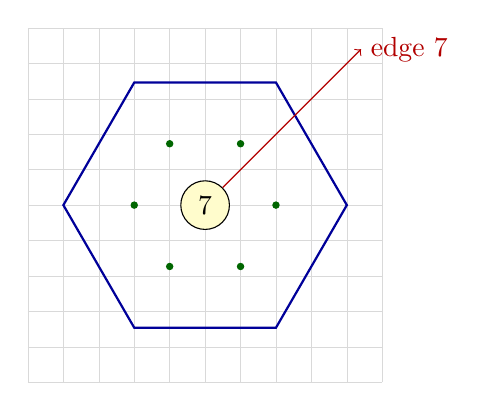
\begin{tikzpicture}[scale=0.9]
    \draw[step=0.5, gray!30, very thin] (-2.5,-2.5) grid (2.5,2.5);
    \draw[thick, blue!60!black] (2.00,0.00) -- (1.00,1.73) -- (-1.00,1.73) -- (-2.00,0.00) -- (-1.00,-1.73) -- (1.00,-1.73) -- cycle;
    \node[draw, circle, fill=yellow!20] (c7) at (0,0) {7};
    \draw[->, red!70!black] (c7) -- (2.2,2.2) node[right] {edge 7};
    \foreach \x in {1,...,6} { \fill[green!40!black] (\x*360/6:1) circle (1.5pt); }
  \end{tikzpicture}
  \caption{TikZ figure 7.}
  \label{fig:tikz:7}
\end{figure}

Paragraph after figure 7, referring to Figure~\ref{fig:tikz:7}.

\section{Figure 8}
Paragraph before figure 8. The picture below is drawn with TikZ: a regular
polygon with 7 sides, a grid, a labelled node and an arrow.

\begin{figure}[h]
  \centering
  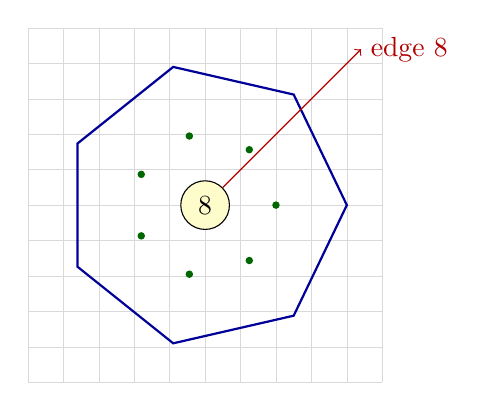
\begin{tikzpicture}[scale=0.9]
    \draw[step=0.5, gray!30, very thin] (-2.5,-2.5) grid (2.5,2.5);
    \draw[thick, blue!60!black] (2.00,0.00) -- (1.25,1.56) -- (-0.45,1.95) -- (-1.80,0.87) -- (-1.80,-0.87) -- (-0.45,-1.95) -- (1.25,-1.56) -- cycle;
    \node[draw, circle, fill=yellow!20] (c8) at (0,0) {8};
    \draw[->, red!70!black] (c8) -- (2.2,2.2) node[right] {edge 8};
    \foreach \x in {1,...,7} { \fill[green!40!black] (\x*360/7:1) circle (1.5pt); }
  \end{tikzpicture}
  \caption{TikZ figure 8.}
  \label{fig:tikz:8}
\end{figure}

Paragraph after figure 8, referring to Figure~\ref{fig:tikz:8}.

\section{Figure 9}
Paragraph before figure 9. The picture below is drawn with TikZ: a regular
polygon with 8 sides, a grid, a labelled node and an arrow.

\begin{figure}[h]
  \centering
  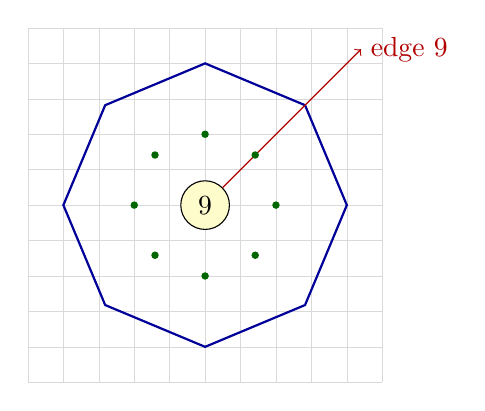
\begin{tikzpicture}[scale=0.9]
    \draw[step=0.5, gray!30, very thin] (-2.5,-2.5) grid (2.5,2.5);
    \draw[thick, blue!60!black] (2.00,0.00) -- (1.41,1.41) -- (0.00,2.00) -- (-1.41,1.41) -- (-2.00,0.00) -- (-1.41,-1.41) -- (-0.00,-2.00) -- (1.41,-1.41) -- cycle;
    \node[draw, circle, fill=yellow!20] (c9) at (0,0) {9};
    \draw[->, red!70!black] (c9) -- (2.2,2.2) node[right] {edge 9};
    \foreach \x in {1,...,8} { \fill[green!40!black] (\x*360/8:1) circle (1.5pt); }
  \end{tikzpicture}
  \caption{TikZ figure 9.}
  \label{fig:tikz:9}
\end{figure}

Paragraph after figure 9, referring to Figure~\ref{fig:tikz:9}.

\section{Figure 10}
Paragraph before figure 10. The picture below is drawn with TikZ: a regular
polygon with 4 sides, a grid, a labelled node and an arrow.

\begin{figure}[h]
  \centering
  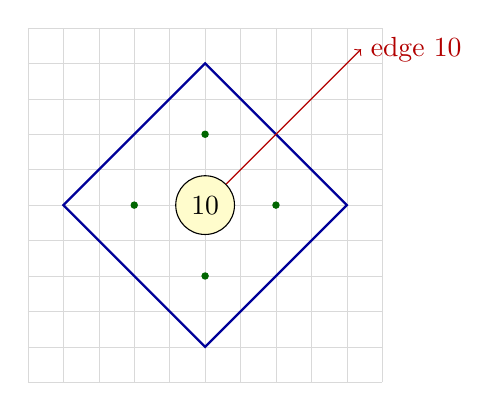
\begin{tikzpicture}[scale=0.9]
    \draw[step=0.5, gray!30, very thin] (-2.5,-2.5) grid (2.5,2.5);
    \draw[thick, blue!60!black] (2.00,0.00) -- (0.00,2.00) -- (-2.00,0.00) -- (-0.00,-2.00) -- cycle;
    \node[draw, circle, fill=yellow!20] (c10) at (0,0) {10};
    \draw[->, red!70!black] (c10) -- (2.2,2.2) node[right] {edge 10};
    \foreach \x in {1,...,4} { \fill[green!40!black] (\x*360/4:1) circle (1.5pt); }
  \end{tikzpicture}
  \caption{TikZ figure 10.}
  \label{fig:tikz:10}
\end{figure}

Paragraph after figure 10, referring to Figure~\ref{fig:tikz:10}.

\section{Figure 11}
Paragraph before figure 11. The picture below is drawn with TikZ: a regular
polygon with 5 sides, a grid, a labelled node and an arrow.

\begin{figure}[h]
  \centering
  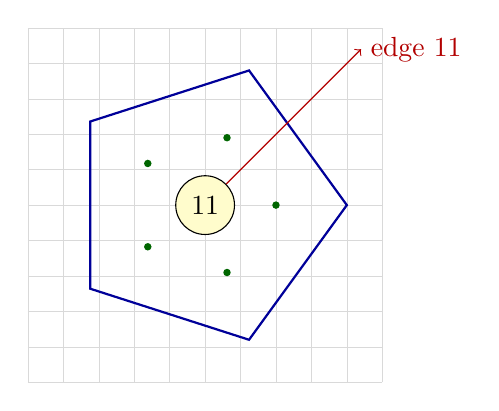
\begin{tikzpicture}[scale=0.9]
    \draw[step=0.5, gray!30, very thin] (-2.5,-2.5) grid (2.5,2.5);
    \draw[thick, blue!60!black] (2.00,0.00) -- (0.62,1.90) -- (-1.62,1.18) -- (-1.62,-1.18) -- (0.62,-1.90) -- cycle;
    \node[draw, circle, fill=yellow!20] (c11) at (0,0) {11};
    \draw[->, red!70!black] (c11) -- (2.2,2.2) node[right] {edge 11};
    \foreach \x in {1,...,5} { \fill[green!40!black] (\x*360/5:1) circle (1.5pt); }
  \end{tikzpicture}
  \caption{TikZ figure 11.}
  \label{fig:tikz:11}
\end{figure}

Paragraph after figure 11, referring to Figure~\ref{fig:tikz:11}.

\section{Figure 12}
Paragraph before figure 12. The picture below is drawn with TikZ: a regular
polygon with 6 sides, a grid, a labelled node and an arrow.

\begin{figure}[h]
  \centering
  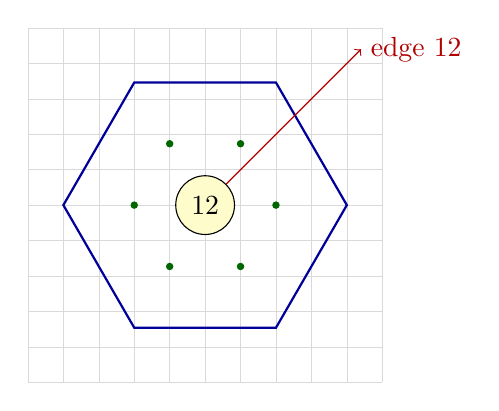
\begin{tikzpicture}[scale=0.9]
    \draw[step=0.5, gray!30, very thin] (-2.5,-2.5) grid (2.5,2.5);
    \draw[thick, blue!60!black] (2.00,0.00) -- (1.00,1.73) -- (-1.00,1.73) -- (-2.00,0.00) -- (-1.00,-1.73) -- (1.00,-1.73) -- cycle;
    \node[draw, circle, fill=yellow!20] (c12) at (0,0) {12};
    \draw[->, red!70!black] (c12) -- (2.2,2.2) node[right] {edge 12};
    \foreach \x in {1,...,6} { \fill[green!40!black] (\x*360/6:1) circle (1.5pt); }
  \end{tikzpicture}
  \caption{TikZ figure 12.}
  \label{fig:tikz:12}
\end{figure}

Paragraph after figure 12, referring to Figure~\ref{fig:tikz:12}.

\end{document}
